\newpage
\clearpage

\section{Investigation}
\label{sec:investigation}

To investigate such reciprocal sharing opportunities, we obtained a \wifi{} scan
result dataset from \PhoneLab{} (\S\ref{subsec:phonelab}). We first discuss some
heuristics to identify the home AP for each device
(\S\ref{subsec:homeap}). Then we show the RSSI comparison between a user's home
and neighbor APs (\S\ref{subsec:better}). Finally, we explore the reciprocal
sharing relationships in the dataset (\S\ref{subsec:reciprocal}).

\subsection{PhoneLab \wifi{} Dataset}
\label{subsec:phonelab}

\begin{table}[t]
  \begin{tabularx}{\columnwidth}{Xr}
    \toprule
    Begin & 11/7/2014 \\ 
    End & 4/3/2015 \\ 
    Duration (Days) & 147 \\ \midrule
    Participants & 254 \\
    Device Type & Nexus~5 \\ \midrule
    Scans & \num{21192417} \\
    Observed APs & \num{1197522} \\
    Used APs & \num{15668} \\ \midrule
    \wifi{} Sessions & \num{466032} \\
    \bottomrule
  \end{tabularx}
  \caption{\textbf{\PhoneLab{} \wifi{} Dataset Summary.} Used APs refers to the
  subset of total APs that were used by the devices participating in the study.}
  \label{tab:summary}
\end{table}

\PhoneLab{}\cite{phonelab-sensemine13} is a public smartphone platform testbed
operated at the University at Buffalo. Several hundreds of participants carry
instrumented Nexus 5 smartphones as their primary device. In particular, the
smartphone platform was modified to log each \wifi{} scan result as well as
connection events naturally generated by the Android system. Note that the same
information can also also be collected by applications with appropriate permissions.
Table~\ref{tab:summary} summarizes the \PhoneLab{} \wifi{} dataset.

A \wifi{} scan result represents the device's network visibility, and consists of
multiple entries---each corresponds to one \wifi{} AP the device
observed. The content of one entry includes: (1) beacon timestamp, (2) AP SSID
and BSSID, (3) AP channel and (4) RSSI. Additionally, the timestamp when the
scan was performed is also logged.

\subsection{Home AP Detection}
\label{subsec:homeap}

We focus on home \wifi{} networks which are more likely to reveal stable and
immediate reciprocal sharing opportunities. For this purpose, we first developed
several heuristics to identify the home AP for each device in the dataset. The
intuition is that the devices are most likely connected to their home AP at
night. More specifically, to identify the home AP for a device, we look at
\wifi{} sessions that happened during 12~AM and 4~AM and count the number of
days that the device connects to each AP during this time period. We then
identify the AP which has the largest day count as the device's home AP,
provided that the day count is larger than a threshold (30 days).

After applying the above heuristics, the home AP information of 107 devices are
identified, including 101 unique BSSIDs. There are 6 BSSIDs that are identified
as home APs for two devices. After further investigation and clarification with
\PhoneLab{} administrators, we found this is because some participants are family
members, and certain participants had device replacements during the data
collection period. In both cases, multiple devices may be associated with the
same home AP.

\subsection{\wifi{} Session Signal Strength}
\label{subsec:better}

After identifying the home AP for each device, we ask two questions: (1) When
the device is connected to its home AP, how often does it receive a better signal
from neighbors' APs which it does not have access to? and (2) When the home AP
fails to provide the best signal, is there one dominant neighbor AP 
that provides better signal most of the time?

\sloppy{%
  To answer the first question, we inspect scan results that are reported during
  \wifi{} sessions with home APs. For each such scan result, we identify the
  currently associated home AP, $AP_{home}$, and the AP with best RSSI among all
  reported APs, denoted as $AP_{best}$. We are particularly interested in
  \textit{sub-optimal} cases, where: (1) $AP_{home} \neq AP_{best}$; (2) the
  device never connects to $AP_{best}$ in the dataset; and (3) the RSSI of
  $AP_{best}$ is better than $AP_{home}$ by at least a certain threshold (5~dBm
  in our analysis). Such cases indicate that the device could potentially
  improve its \wifi{} performance by connecting to a neighbor AP which has a
  strong signal yet it does not have access to that AP. Note that here we
  consider RSSI as a hint in determining the \textit{optimal} AP and it is well
  understood that RSSI does not directly translate to \wifi{} performance, which
  we will discuss in Section~\ref{sec:challenges}.  Also note that the cases
  when the device is not connected to APs with the strongest signal due to bad
  roaming strategies are not interesting in the context of this paper, and are
  excluded by the second condition.
}

\begin{figure}[t]
  \centering
  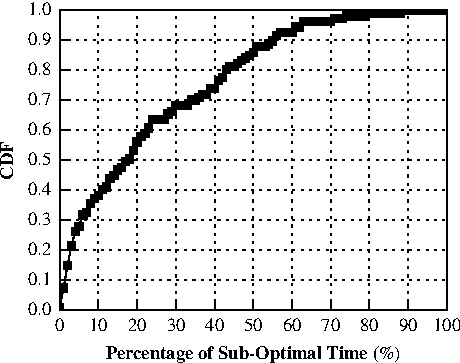
\includegraphics[width=\columnwidth]{./figures/HomeAPSessionRSSI.pdf}
  \caption{\textbf{CDF of Sub-Optimal Connection Time.}}
  \label{fig:suboptimal}
\end{figure}

We classify all scan results reported during \wifi{} sessions with home APs into
two categories: sub-optimal and the rest. For each device, we calculate the
percentage of time when the scan results indicate sub-optimal association.
Figure~\ref{fig:suboptimal} shows the CDF of this percentage for 
the 107 devices. We make several observations. First, for 80\% of the devices,
their home APs usually provides best signal (sub-optimal percentage less than
25\%). This result is not particularly surprising considering that home APs are
usually carefully positioned to provide good coverage. Second, we notice
that for certain number (8\%) of devices, their home APs failed to provide best
signal for more than 40\% of the time, suggesting that these users may benefit
from sharing the \wifi{} access of their neighbor APs.

Next, we want to answer the question when the device is in a sub-optimal association
with its home AP, is there a \textit{dominant} neighbor AP that
usually provides the best signal among other neighbor APs? If such dominant
neighbor AP exists, then by just sharing access of this one particular neighbor
AP, the device's sub-optimal association time can be largely reduced. To this
end, we look at all the scan results in the sub-optimal category, and count the
number of times that each neighbor AP appears as $AP_{best}$. For each device,
we calculate the fraction of the dominant neighbor AP. Figure~\ref{fig:dominantap}
shows the CDF of dominant AP fraction. For 50\% of the devices, one particular
neighbor AP contributes to more than 57\% of sub-optimal connection time,
implying that even by sharing \wifi{} access of one neighbor AP, these device's
sub-optimal connection time can be reduced by more than 57\%.

\begin{figure}[t]
  \centering
  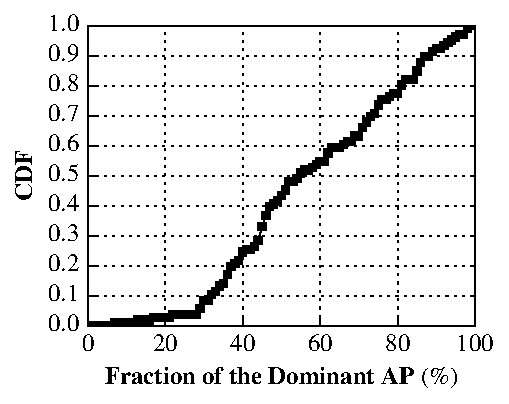
\includegraphics[width=\columnwidth]{./figures/BetterNeighborAPFigure.pdf}
  \caption{\textbf{CDF of Dominant AP Fraction.}}
  \label{fig:dominantap}
\end{figure}


\subsection{Reciprocal Sharing Opportunities}
\label{subsec:reciprocal}

Finally, we investigate the cases where two devices can obtain better signals
from each other's home AP, i.e., reciprocal sharing opportunities. We first use
scan results to establish physical neighbor information between the home APs.
Then we investigate whether reciprocal sharing opportunities exist between
neighbor APs.

To obtain the physical neighbor information, we build a home AP neighbor graph
$G_{neighbor}=(V, E)$, where $V$ is the set of all home APs, and $\langle AP_i,
AP_j \rangle \in E$ if $AP_i$ and $AP_j$ appear in the same result and both AP's
signal strengths are larger than a threshold (80~dBm), meaning $AP_i$ and $AP_j$
are physically colocated with each other. Figure 3 shows the constructed $G_{neighbor}$
from the dataset, where nodes with no edges are omitted. There are three clear
clusters of home APs. We also verified that APs in the same cluster have
different SSID and manufacturer, confirming that they are not centrally deployed
or managed.

Next, we look into potential AP sharing opportunities among colocated APs. For
each edge $\langle AP_i, AP_j \rangle \in E$, if $AP_i$'s clients receive better
(by at least 5~dBm) signal  from $AP_j$, then we draw a directed edge $\langle
AP_i\rightarrow AP_j \rangle}$, indicating that $AP_i$'s clients could
potentially benefit from sharing access of $AP_j$. We also assign a weight to
each directed edge to indicate how often such relationship happens in the
dataset.

The updated home AP neighbor graph is shown in Figure~\ref{fig:reciprocal}.
Sharing opportunities are sparse but exist. In particular, we observe one pair
of home APs, node 12 and 1, which exhibit \textit{reciprocal} sharing
relationships.

\sloppy{%
  We must note that \PhoneLab{} participants reside sparsely among the vast
  Buffalo area, and the above analysis is further restricted to those 
  participants that we can detect their home APs using heuristics described
  Section~\ref{subsec:homeap}. The fact that reciprocal sharing opportunities
  exist at all in such a sparse dataset is quite surprising, and motivates the
  need for a system to detect and enable such reciprocal \wifi{} sharing.
}

\begin{figure}[t]
  \centering
  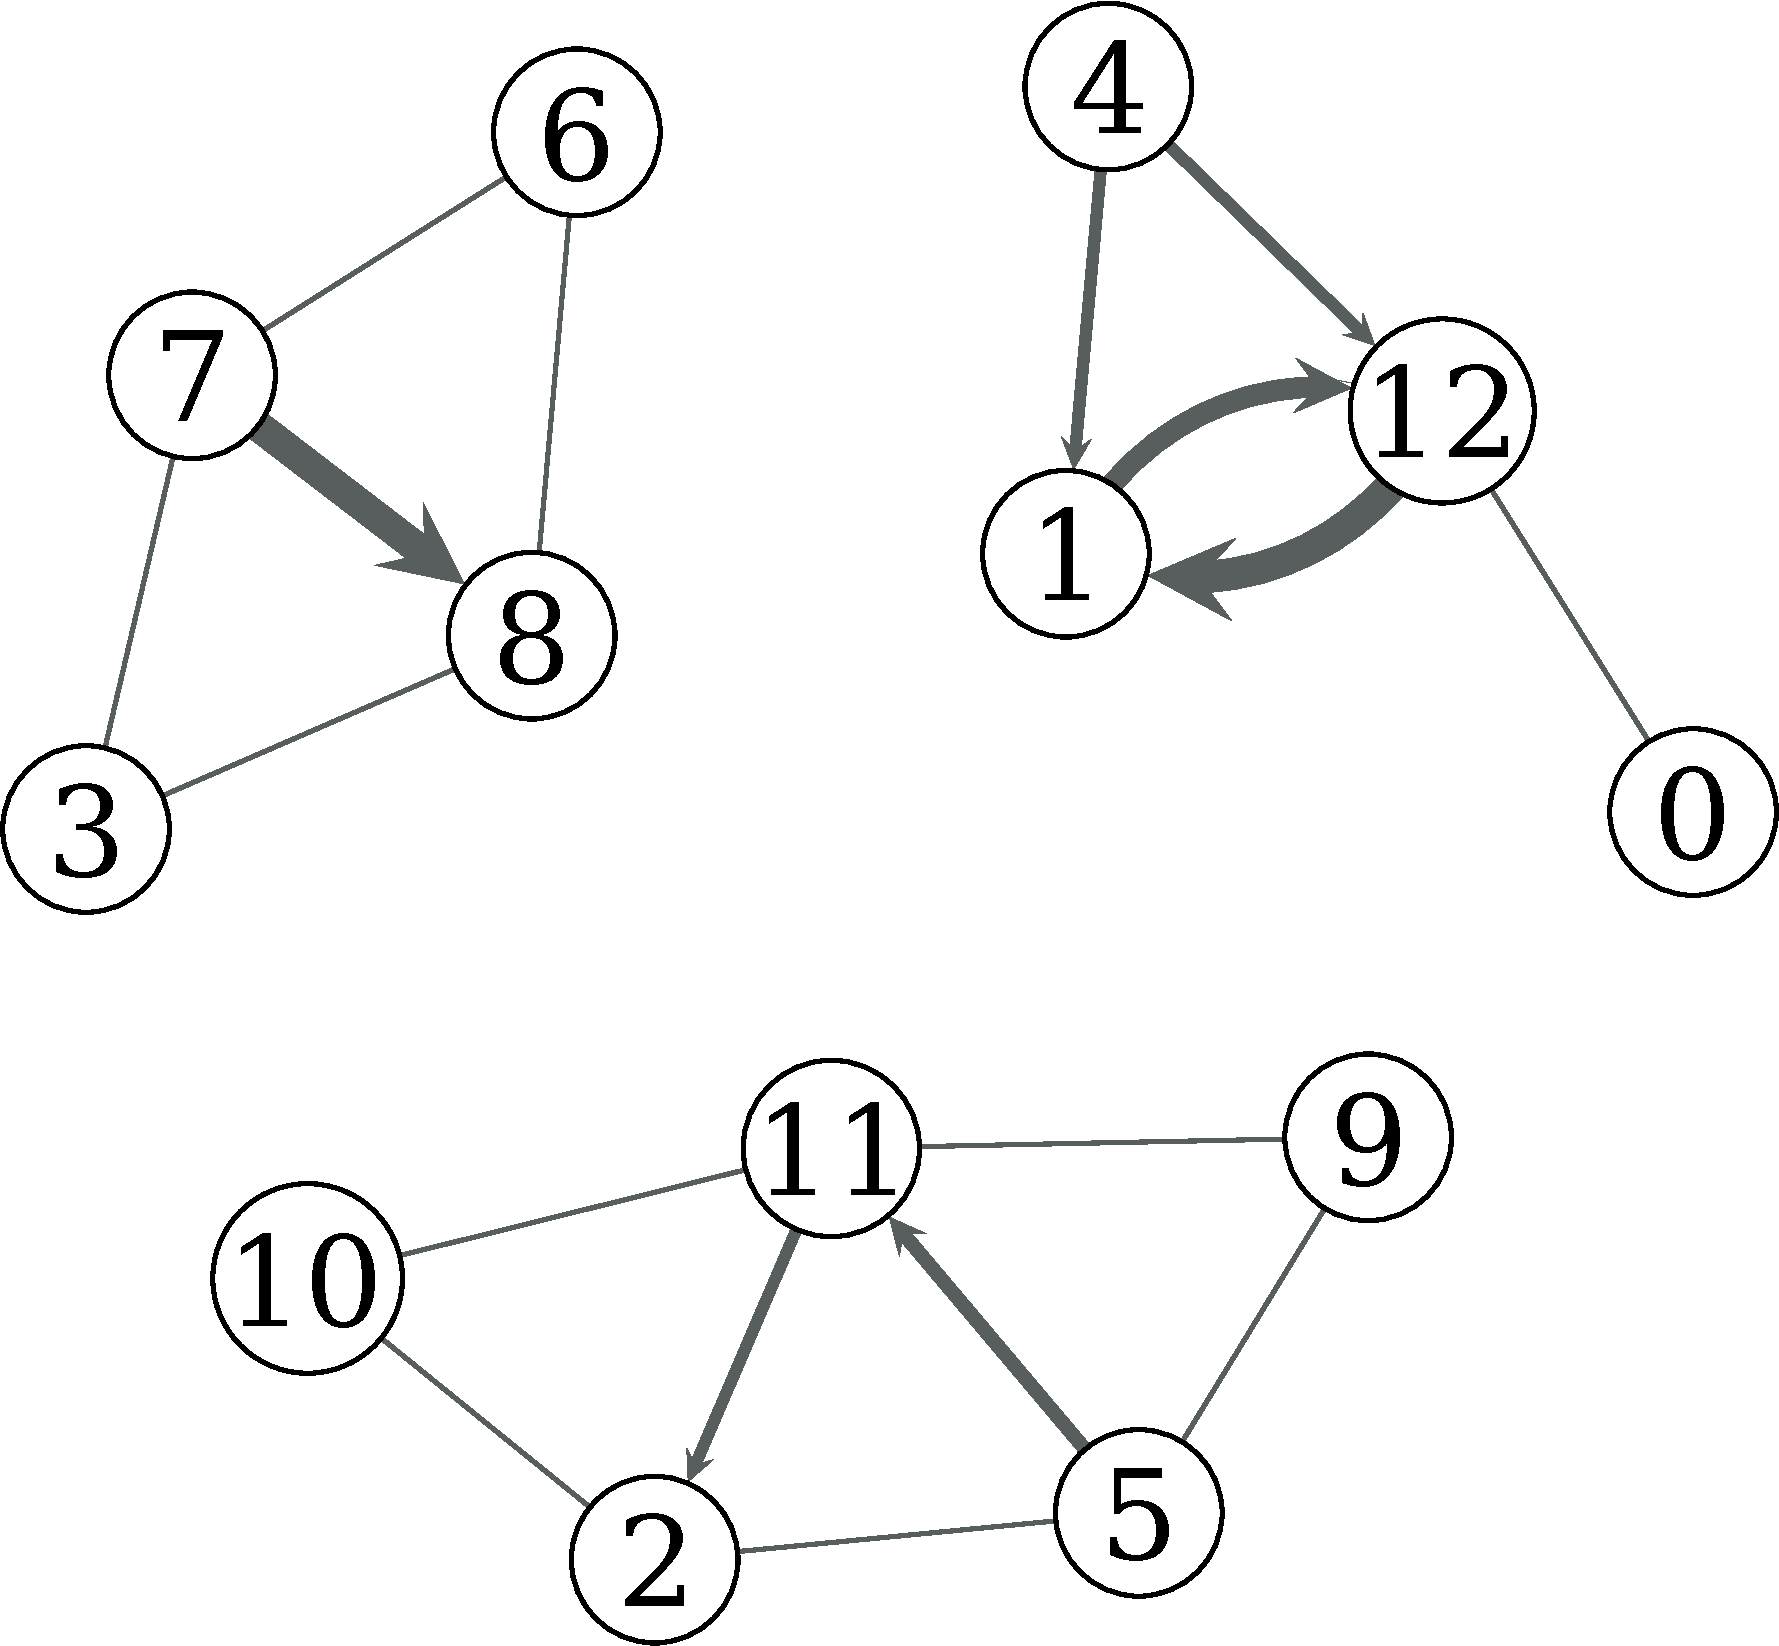
\includegraphics[width=\columnwidth]{./figures/HomeAPNeighborFigure.pdf}
  \caption{\textbf{AP Neighbor and Sharing Graph.} Edges (both directed and
    undirected) denote AP physical
    colocation relationship. Directed edges indicate AP sharing opportunities.
  Thickness of directed edges corresponds to edge weights.}
  \label{fig:reciprocal}
\end{figure}
